\documentclass[10pt,twoside, fleqn]{memoir}
\usepackage{graphicx}
\usepackage{hyperref} % HYPERLINKS
\usepackage[nomain,acronym,toc]{glossaries}
\makeglossaries
\usepackage{xcolor}
\hypersetup{
    colorlinks,
    linkcolor={blue!50!black},
    citecolor={blue!50!black},
    urlcolor={blue!80!black}
}
\definecolor{warningbackground}{RGB}{252,226,158}
\definecolor{infobackground}{RGB}{217,237,247}
\definecolor{infoforeground}{RGB}{58,135,173}
\definecolor{infoborder}{RGB}{188,232,241}
\usepackage{environ}
\usepackage{tikz}
\usetikzlibrary{fit,backgrounds,calc}

%\usepackage[T1]{fontenc}
%\usepackage{mathpazo} % USE PALATINO FONT
%\usepackage[latin1]{inputenc}
%\usepackage[xindy]{imakeidx}

%\usepackage[british]{babel}
%\usepackage[framed, numbered, autolinebreaks]{mcode}
%\usepackage{listings}

%

%\usepackage[font=footnotesize]{caption}
%\usepackage{subcaption}
%\usepackage{pdflscape} %Landscape pages
%\usepackage{pdfpages}
%\usepackage{amsmath}
%\usepackage{amssymb}
%\usepackage{gensymb} %Degree sign
%\usepackage{footnote} %Footnotes in tabulars
%\usepackage{xcolor,framed,marginnote,blindtext}
%\colorlet{shadecolor}{blue!10}
%
%
%\usepackage{tikz} %TO CREATE BLOCK DIAGRAMS
%%\usetikzlibrary{external}
%%\tikzexternalize
%%\tikzset{external/mode=graphics if exists}
%
%\usetikzlibrary{shapes,arrows}
%\usetikzlibrary{positioning}
%
%\setcounter{tocdepth}{2} % DEPTH OF TABLE OF CONTENTS; 2= SUBSECTIONS INCLUDED
%\setcounter{secnumdepth}{2} % SUBSECTIONS ARE NUMBERED
%
%\usetikzlibrary{positioning}



%% BEGIN TITLE

\makeatletter
\def\maketitle{%
  \null
  \thispagestyle{empty}%
  \vfill
  \begin{center}\leavevmode
    \normalfont
    {\LARGE\raggedleft \@author\par}%
    \hrulefill\par
    {\huge\raggedright \@title\par}%
    \vskip 1cm
%    {\Large \@date\par}%
  \end{center}%
  \vfill
  \null
  \cleardoublepage
  }
\makeatother
\author{RYMAPT}
\title{Ethoscope user manual and documentation}
\date{23 February 2015}


\newacronym{ddye}{D$_{\text{dye}}$}{donor dye, ex. Alexa 488}
\newacronym[description={\glslink{r0}{F\"{o}rster distance}}]{R0}{$R_{0}$}{F\"{o}rster distance}
\newglossaryentry{r0}{name=\glslink{R0}{\ensuremath{R_{0}}},text=F\"{o}rster distance,description={F\"{o}rster distance, where 50\% ...}, sort=R}
\newglossaryentry{kdeac}{name=\glslink{R0}{\ensuremath{k_{DEAC}}},text=$k_{DEAC}$, description={is the rate of deactivation from ... and emission)}, sort=k}

% A
\newacronym{af}{AF}{Auto Focus}
\newacronym{apt}{APT}{Advanced Positioning Technology}

% C
\newacronym{ccd}{CCD}{Charge Coupled Device}

% D
\newacronym{dio}{DIO}{Digital InputOutput}
\newacronym{dpss}{DPSS}{Diode Pump Solid State}

% F
\newacronym{fov}{FOV}{Field of View}

% G
\newacronym{gui}{GUI}{Graphic User Interface}

% I
\newacronym{ide}{IDE}{Integrated Development Environment}
\newacronym{ifd}{IFD}{Image File Directory}
\newacronym{ir}{IR}{Infra-red}

% L
\newacronym{led}{LED}{Light Emitting Diode}
\newacronym{lsm}{LSM}{Laser Sheet Microscopy}

% M
\newacronym{mosfet}{MOSFET}{Metal Oxyde Semiconductor Field-Effect Transistor }

% N
\newacronym{nas}{NAS}{Network Attached Storage}
\newacronym{ntc}{NTC}{Negative Temperature Coefficient}

% P
\newacronym{pcb}{PCB}{Printed Circuit Board}
\newacronym{pwm}{PWM}{Pulse Width Modulation}
\newacronym{psf}{PSF}{Point Spread Function}

% S
\newacronym{scl}{SCL}{Serial Clock Line}
\newacronym{sda}{SDA}{Serial DAta line}
\newacronym{shr}{SHR}{Synology Hybrid Raid}
\newacronym{svn}{SVN}{Apache SubVersion}

% T
\newacronym{tif}{TIFF}{Tagged Image File Format}
\newacronym{tps}{TPS}{Thinnest Part of the Sheet}

% U
\newacronym{usb}{USB}{Universal Serial Bus}

% R
\newacronym{roi}{ROI}{Region Of Interest} 


%%% BEGIN DOCUMENT
\makeindex
\begin{document}

\let\cleardoublepage\clearpage


\maketitle
\frontmatter

\null\vfill
\begin{center}
\begin{figure}
  \centering
  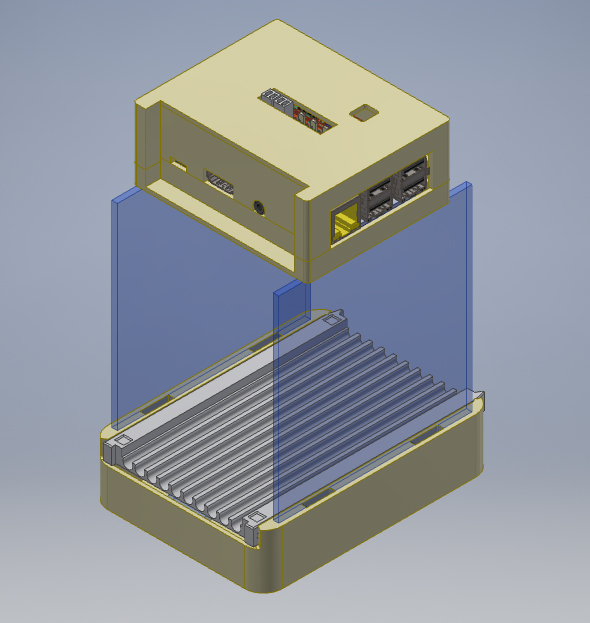
\includegraphics[width=0.80\textwidth]{./images/isometric.jpg}
  \label{fig:Intro}
\end{figure}
\end{center}
\begin{flushleft}
\textit{Ethoscope user manual and documentation}\newline
\newline
RYMAPT - 2017\newline info@rymapt.com
\bigskip

\end{flushleft}
\let\cleardoublepage\clearpage

\newpage
\tableofcontents

\mainmatter
\sloppy

\newenvironment{SpecialPar}
  {\begin{shaded}\marginnote{\fbox{NOTE}}}
  {\end{shaded}}

%%%%%%%%%%%%%%%%%%%%%%%
% COMMAND TO CREATE A WARNING BOX
\NewEnviron{alertinfo}[1]
{
    \begin{tikzpicture}
    \node[inner sep=0pt,
          draw=infoborder,
          line width=1.2pt,
          fill=infobackground] (box) {\parbox[t]{.99\textwidth}
        {%
            \begin{minipage}{.15\textwidth}
                \centering\tikz[scale=3]
                \node[scale=1]
                {
                    
\includegraphics[scale=0.04]{./images/warning.png}
                };
            \end{minipage}%
           \begin{minipage}{.80\textwidth}
                \vskip 10pt
                \textbf{\textcolor{infoforeground}{#1}}\par\smallskip
                \textcolor{infoforeground}{\BODY}
                \par\smallskip
            \end{minipage}\hfill
        }%
    };

    \end{tikzpicture}
}
%%%%%%%%%%%%%%%%%%%%%%%


%%% INCLUDE CHAPTERS
%\include{ch_Introduction}
\chapter{Hardware description}\label{ch:hardware}
The Ethoscope is comprised of the following parts:
\begin{description}
  \item[Top unit] This contains the main components of the Ethoscope, such as the processing unit, the camera and the environmental shield (optional). The components are enclosed in a plastic shell.
  \item[Base unit] The unit acts as a base for the whole Ethoscope and as a support and alignment tool for the arena. The base unit also contains the strip of \gls{led} used to provide \gls{ir} illumination to the arena.
  \item[Arena] The arena defines the experiment to be performed. The basic arena, provided with the standard kit, provides support for up to twenty glass tubes, each one defined as a \gls{roi}. Three black dots in the corner of the arena are used by the software to determine a spatial system of reference.
  \item[Side walls] The walls connect the base to the top unit and ensure a correct distance between camera and arena. The standard walls are made of 3~mm acrylic sheet.
\end{description}

\section{Setup}\label{ch:setup}
 
%\include{ch_MainGUI}
%\include{ch_Calibration}
%\include{ch_Tracking}
%\include{ch_PSF}

%%% APPENDIX
%\include{ch_Appendix}


%%% GLOSSARY
%\printglossaries
%\printglossary[type=\acronymtype]
\printglossary[type=\acronymtype,title=Abbreviations]

%%% BIBLIOGRAPHY
%\bibliographystyle{unsrt}
%\bibliography{./../Bibliography/myBibliography}


\end{document} 